The six targets all concern prostate cancer, but they occupy different biological and
clinical levels and therefore cannot be interpreted as interchangeable pathology features.
They are Grade/ISUP, tumor phenotype/content, PTEN loss, AR activity, SPOP mutation, and
recurrence.
The primary result is their comparative evidence hierarchy; no single target serves as a
surrogate for the other five. ISUP is highlighted later only because it reached an additional
functional-sensitivity experiment.
Every numerical alignment result used an available target-specific reference paired to the
slide-derived embedding at the registered analysis unit. Unequal reference coverage limited
which external, conditional, or functional questions could be asked; it was not converted
into a negative association. Thus, not evaluated or blocked denotes a missing prerequisite,
whereas unsupported denotes an available comparison that did not qualify the proposed
signal. SPOP belongs to the latter category; phenotype functional testing and molecular
external transport illustrate the former.
Table~\ref{tab:alignment-summary} presents the study's headline evidence states and the
permitted interpretation of each candidate coordinate. The Introduction provides the concise
clinical orientation; Supplementary Section S1 retains the detailed target, paired-reference,
availability, metric, and six-axis biological definitions and separates representation
evidence from functional evidence about the BCR head.

\begin{table}[H]
\centering
\footnotesize
\setlength{\tabcolsep}{3pt}
\renewcommand{\arraystretch}{1.18}
\caption{Evidence-qualified candidate shared coordinates. States summarize the available axis-specific evidence: transportable means directional external transfer was retained; context-sensitive means interpretation narrowed under a clinical, site, representation, sampling, or endpoint audit; unsupported means the frozen primary design did not qualify the signal. Functional use refers specifically to intervention on a locked BCR head and is not implied by recoverability.}
\label{tab:alignment-summary}
\begin{tabular}{@{}>{\raggedright\arraybackslash}p{0.15\textwidth}>{\raggedright\arraybackslash}p{0.16\textwidth}>{\raggedright\arraybackslash}p{0.38\textwidth}>{\raggedright\arraybackslash}p{0.23\textwidth}@{}}
\toprule
Target & State & Permitted interpretation & Functional use \\
\midrule
Grade/ISUP & Transportable & Grade information is recoverable and directionally transports across compatible external resources & Internal exploratory locked-BCR-head sensitivity; site evidence encoder-specific and LEOPARD external gate failed or remained inconclusive \\
Tumor phenotype/content & Transportable & Morphology-linked phenotype is recoverable and transports directionally; the external target is grade-derived tumor/benign status, not exact tumor-content truth & Currently blocked: same-cohort independent tumor-content truth unavailable \\
PTEN & Context-sensitive & PTEN-related information is recoverable within TCGA-PRAD but grade-independent increment and external transport are not established & Feasible follow-up; not run \\
AR activity & Context-sensitive & AR activity has positive pooled alignment but grade-independent increment and site transport remain unresolved & Feasible follow-up; not run \\
SPOP & Unsupported (frozen design) & Evaluated against an available genomic reference, but no reliable frozen-design signal was established & Not qualified: recoverability unsupported \\
Recurrence & Context-sensitive & Recurrence alignment is endpoint representation and covariate hierarchy conditioned & Not applicable as input erasure; prognostic validation required \\
\bottomrule
\end{tabular}
\end{table}


\subsection{The study separates recoverability, reproducibility, and functional use}

\paragraph{Alignment question.}
What evidence is required before a human-defined target can be used to interpret an AI
representation, and which stronger conclusions remain outside that evidence?

\paragraph{Analysis frame.}
We organized each target by the evidence needed to use it as a human--AI interpretive
coordinate (Figure~\ref{fig:alignment-map}). A target first had to be recoverable from a
frozen representation at its registered analysis unit. External application without
target-cohort refitting evaluated transport where compatible labels existed. Conditional,
site, representation, and endpoint audits then identified restrictions. Unevaluated axes
remained missing evidence rather than negative findings.

\paragraph{Evidence test.}
The test was not whether one metric exceeded a universal cutoff. Instead, the registered
target was followed across the available evidence axes, with its cohort, analysis unit,
metric, null, and uncertainty retained. External transport required an unchanged source
probe; conditional increment required a held-out comparison with a clinical reference;
site, setting, and endpoint audits addressed different alternative explanations.

\paragraph{Interpretive boundary.}
This structure produced three manuscript-facing states: transportable,
context-sensitive, and unsupported in the frozen design. These are target-specific evidence
states, not model confidence scores or clinical action thresholds. Recoverability and
transport occupy the left side of the evidence chain. For grade, a separate internal FM6
analysis used locked BCR heads, target-specific erasure, and matched controls to test a
narrow functional-sensitivity claim. The other targets have different functional-evidence
states: phenotype is blocked by unavailable same-cohort independent truth; PTEN and AR are
feasible follow-up analyses that were not run; SPOP lacks a qualified recoverable direction;
and recurrence is the outcome predicted by the head rather than an input target for erasure.
External functional replication was not achieved.

\paragraph{Qualification rule.}
A target was called transportable only when an appropriate external evaluation retained a
consistent direction without target-cohort refitting. Context-sensitive means that the
interpretation materially depended on grade, site, representation, sampling, or endpoint.
Unsupported means that the frozen primary design did not support the proposed effect; it
does not mean that the biology is absent. Missing axes remain not evaluated.

\begin{figure}[H]
\centering
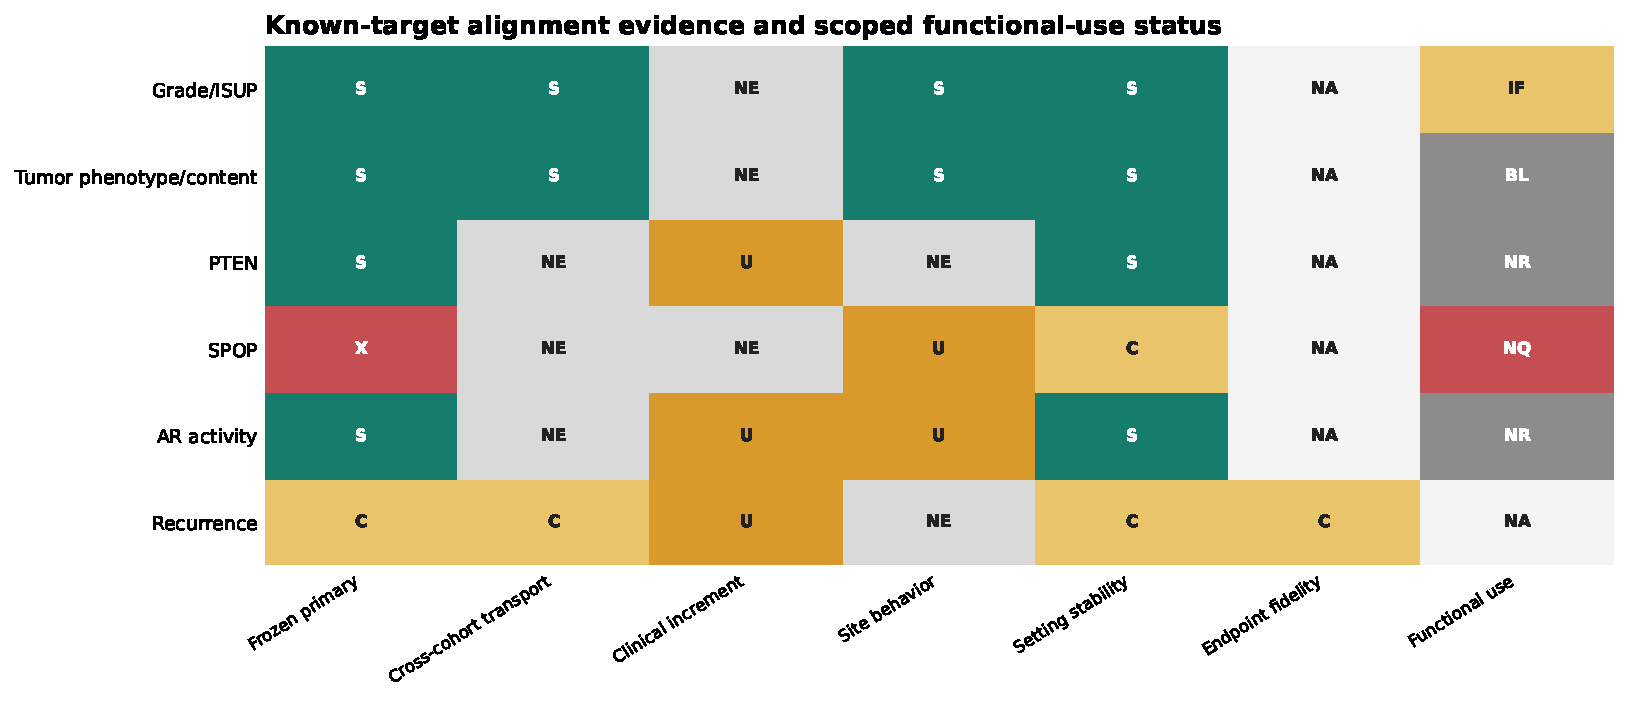
\includegraphics[width=\textwidth]{figures/fig1_alignment_map.pdf}
\caption{\textbf{Evidence-qualified map of candidate shared interpretive coordinates.}
Rows are clinically interpretable targets and columns are distinct evidence axes. A
supported cell means only that the named axis was supported. Unresolved, not evaluated,
and not applicable cells are preserved. Cell codes are S, supported; C, context-sensitive;
U, unresolved; NE, not evaluated; NA, not applicable; and X, unsupported in the frozen
design. In the final column, IE denotes internal exploratory functional sensitivity for
grade; BL, blocked because same-cohort independent phenotype truth was unavailable; NR,
feasible but not run for PTEN and AR; NQ, not qualified because SPOP recoverability was
unsupported; and NA, not applicable because recurrence is the predicted outcome. IE does
not mean indispensable, externally reproduced, or clinically incremental use.}
\label{fig:alignment-map}
\end{figure}

\paragraph{How to read the qualification map (Figure~\ref{fig:alignment-map}).}
Read each row from left to right rather than comparing colors vertically as if they were a
model leaderboard. The first cells ask whether the target can be recovered and transported.
The middle cells ask whether that interpretation narrows after clinical, site, technical,
or endpoint checks. A supported cell applies only to the named axis; it does not fill a
missing cell elsewhere. The final functional-use column is deliberately marked as not
one generic ``not tested'' state: it distinguishes a completed internal exploratory test
from an unavailable prerequisite, a feasible analysis not run, an unqualified direction,
and a question that is not applicable. This prevents probe recoverability from being
mistaken for functional evidence and prevents the scoped grade result from being generalized
to other targets.


\subsection{Morphology-linked targets provide the best-qualified candidate coordinates}
\label{sec:results-morphology}

\paragraph{Alignment question.}
Can clinically familiar architectural targets be recovered from frozen representations and
retain their direction when the same probe is applied to independent resources?

\paragraph{Analysis frame.}
Grade and tumor phenotype were evaluated in NADT-Prostate and then transferred without
target-cohort refitting to PANDA; PRECISE supplied a separate session-level grade estimate.
Spearman correlation assessed rank preservation for grade and continuous phenotype, while
AUROC assessed grade-derived benign-versus-tumor discrimination.

\paragraph{Evidence test.}
Grade and phenotype showed the broadest available alignment across cohorts
(Figure~\ref{fig:known-target-alignment}). In NADT-Prostate, the patient-level CONCH grade
probe had Spearman $\rho=0.478$ (patient-bootstrap interval 0.170--0.712; 39 patients), and
the tumor-phenotype signal had $\rho=0.800$ (0.625--0.909; 39 patients). Applied without
target-cohort refitting, the grade probe retained positive associations in PANDA Karolinska
($\rho=0.354$; 565 case images) and Radboud ($\rho=0.519$; 572 case images). The
phenotype probe discriminated grade-derived tumor status in the same institutions with
AUROCs of 0.786 and 0.871. A separate PRECISE evaluation yielded grade
$\rho=0.865$ across 17 imaging sessions.

\paragraph{Interpretive boundary.}
These rows demonstrate directional transport of morphology-linked information, not uniform
precision. Saved target-cohort intervals were unavailable for PANDA and PRECISE and were not
reconstructed. Analysis units also differed across patient, case image, and session. Exact
effect sizes therefore remain specific to the registered cohort and unit. In particular,
the PANDA phenotype target was grade-derived tumor-versus-benign status, not an independent
same-patient measurement of quantitative tumor content. Its result supports directional
transport of a tumor-related phenotype score; it does not show that exact tumor fraction
was reproduced externally.

\paragraph{Qualification rule.}
Grade and phenotype qualify as the strongest transportable candidate coordinates because the
locked source probe retained the expected direction in external resources. This state does
not imply interchangeable effect sizes across datasets, complete representation explanation,
or functional use by a later disease-prediction head.

\begin{figure}[H]
\centering
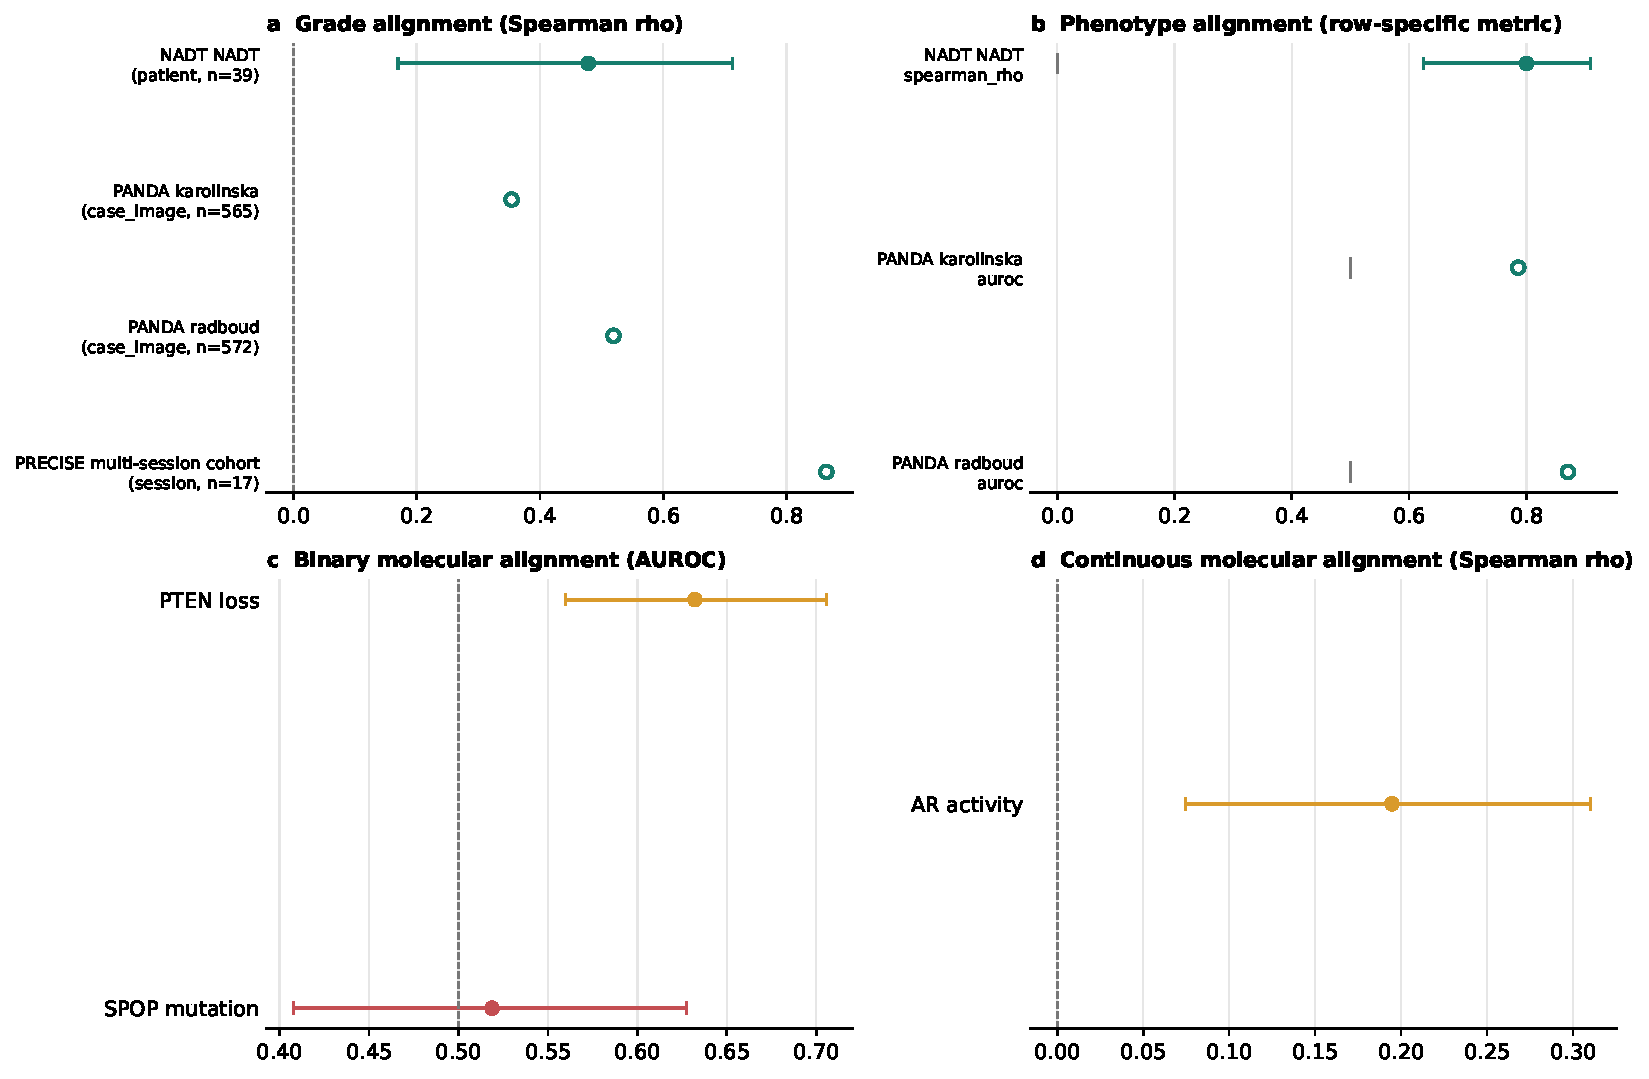
\includegraphics[width=\textwidth]{figures/fig2_known_target_alignment.pdf}
\caption{\textbf{Recoverability and transport of known morphologic and molecular targets.}
\textbf{a}, Grade and phenotype estimates across source and external resources; metrics and
analysis units are displayed rather than pooled. The PANDA phenotype rows use grade-derived
tumor-versus-benign status and therefore test directional phenotype transport, not exact
external tumor-content agreement. \textbf{b}, Frozen-primary molecular alignment in
TCGA-PRAD; these molecular rows are within-cohort recoverability results, not external
transport. Whiskers are shown only where saved patient-bootstrap intervals were available.
Dashed lines mark correlation zero or AUROC chance.}
\label{fig:known-target-alignment}
\end{figure}

The complete ten-row primary evidence frame, including cohort, unit, denominator, metric,
and retained uncertainty, is provided in Supplementary Section S4. It prevents estimates
with different analysis units or precision from being treated as directly interchangeable.


\subsection{Molecular coordinates separate into recoverable, conditional, and unsupported states}
\label{sec:results-molecular}

\paragraph{Alignment question.}
Do frozen histology representations contain information associated with PTEN loss, SPOP
mutation, and AR activity, and does any observed association provide information beyond
grade or remain stable across source sites?

\paragraph{Analysis frame.}
The primary molecular frame comprised 273 TCGA-PRAD patients. PTEN loss and SPOP mutation
were binary targets scored by AUROC; AR activity was continuous and scored by Spearman
correlation. Nested, patient-disjoint models compared image information with grade, while
site and representation audits tested the scope of the pooled association.

\paragraph{Evidence test.}
PTEN loss was recoverable with a frozen-primary CONCH AUROC of 0.632 (0.560--0.706). AR
activity had a positive patient-level Spearman correlation of 0.195 (0.074--0.310). By
contrast, the SPOP frozen-primary AUROC was 0.519 (0.408--0.627), and its broader correlated
seed-cell range crossed chance (0.348--0.679). Conditional audits further narrowed PTEN and
AR (Figure~\ref{fig:conditional-alignment}). The held-out increment beyond grade was
$+0.019$ AUROC ($-0.025$ to $+0.068$) for CONCH PTEN and $+0.035$
($-0.013$ to $+0.087$) for Virchow PTEN. AR increments in $R^2$ were $+0.004$
($-0.036$ to $+0.042$) and $+0.019$ ($-0.015$ to $+0.051$), respectively.
The pooled AR direction was positive, but each of six stored site-specific intervals crossed
zero. The expanded site audit in Figure~\ref{fig:conditional-alignment} also preserves all
evaluable SPOP sites: their intervals included or touched chance, while the CH site contained
no positive event and therefore had undefined AUROC. Site remained entangled with
acquisition and case mix.

\paragraph{Interpretive boundary.}
Recoverable molecular information was not shown to add held-out information beyond grade.
Site codes cannot be given a causal scanner interpretation. None of these results establishes
routine molecular diagnosis from H\&E or functional use of a molecular target by an AI
disease decision. The SPOP genomic reference was available and was used; its unsupported
state is therefore an evaluated lack of qualification in this frozen design, not a missing-
label or not-evaluated result.

\paragraph{Qualification rule.}
PTEN and AR are context-sensitive candidate within-cohort coordinates because primary
recoverability was present but independent increment beyond grade and site transport were
not established. SPOP is unsupported in the frozen primary design because its estimate and
broader setting range did not separate reliably from chance. These states qualify the
present evidence, not the biological existence of the alterations.

\begin{figure}[H]
\centering
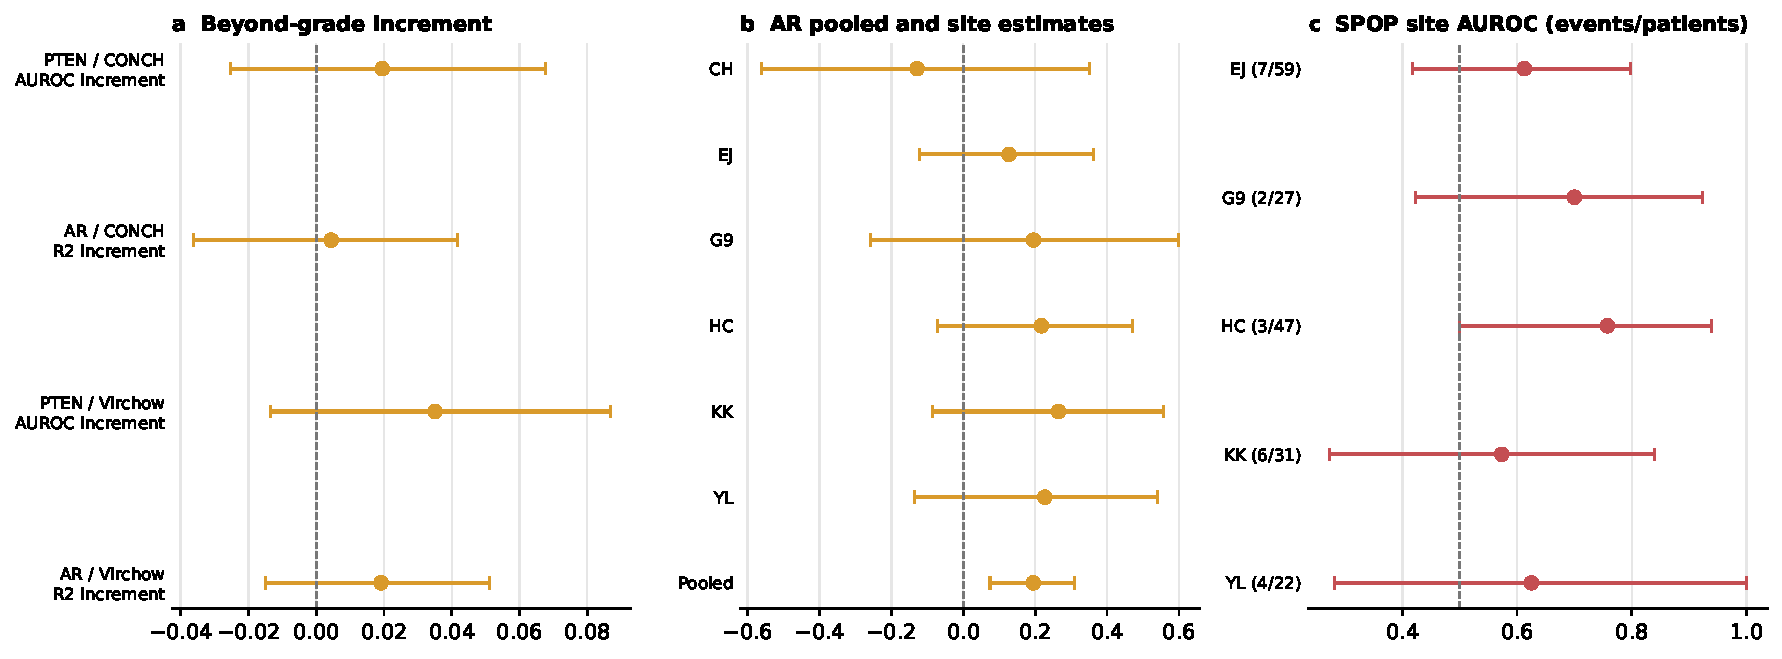
\includegraphics[width=\textwidth]{figures/fig3_conditional_alignment.pdf}
\caption{\textbf{Conditional and site-specific narrowing of molecular alignment.}
\textbf{a}, Held-out PTEN and AR increments beyond grade for CONCH and Virchow.
Positive values indicate improvement after adding the image-derived score to the grade
reference; the row-specific metrics are AUROC for PTEN and $R^2$ for AR.
\textbf{b}, Pooled and site-specific AR correlations. \textbf{c}, SPOP site-specific AUROCs,
with positive-event and patient counts; CH is retained as a single-class, undefined row in
the accompanying source table rather than assigned an AUROC. Intervals crossing or touching
the relevant null indicate unresolved conditional evidence, not absence of biological signal.
PTEN and AR use by a BCR head was not tested. SPOP was tested against an available genomic
reference but did not qualify a stable frozen-representation direction.}
\label{fig:conditional-alignment}
\end{figure}


\subsection{Outcome alignment changes with endpoint and clinical reference}
\label{sec:results-outcome}

\paragraph{Alignment question.}
Does a transferred image-derived recurrence score preserve patient risk ordering, and is
its interpretation stable when the event definition or clinical reference changes?

\paragraph{Analysis frame.}
The post-hoc score was fitted in LEOPARD and applied unchanged to TCGA-PRAD. Concordance was
evaluated separately for reconstructed with-tumor recurrence and official TCGA-CDR PFI.
Increment analyses compared grade alone with grade plus the image score in the same 153
complete cases and the same paired bootstrap draws.

\paragraph{Evidence test.}
In the 270-patient transfer frame, the reconstructed with-tumor endpoint yielded a C-index
of 0.673 (95\% interval 0.587--0.759; 57 events), whereas official PFI yielded 0.586
(0.482--0.689; 42 events). On 153 complete cases, adding the image score to grade changed
C-index by $+0.083$ ($+0.012$ to $+0.157$; 30 reconstructed events), but the paired
integrated Brier-score interval included zero. For official PFI, the C-index increment was
$+0.032$ ($-0.040$ to $+0.126$; 15 events), and all paired official-PFI C-index and
integrated-Brier-score intervals included zero. Fuller clinical and site comparisons did
not establish robust independent increment. The complete same-patient,
same-bootstrap-draw comparison family is reported in Supplementary Section S9; it shows
that interpretation depends on the comparator and performance metric. Figure~\ref{fig:outcome-contrasts}
shows that complete comparison family while retaining separate endpoint panels.

\paragraph{Interpretive boundary.}
Concordance measures risk ordering, not calibrated individual risk or clinical usefulness.
The reconstructed endpoint and official PFI contain different event definitions and event
counts; performance on one cannot be relabelled as performance on the other. The PCA sweep
that generated the post-hoc signal was exploratory rather than an unbiased model-selection
procedure.

\paragraph{Qualification rule.}
Recurrence remains an endpoint-conditioned, context-sensitive exploratory coordinate because
its estimate changed with the endpoint and robust independent increment over clinical
references was not established. It is not a validated prognostic biomarker.

\begin{figure}[H]
\centering
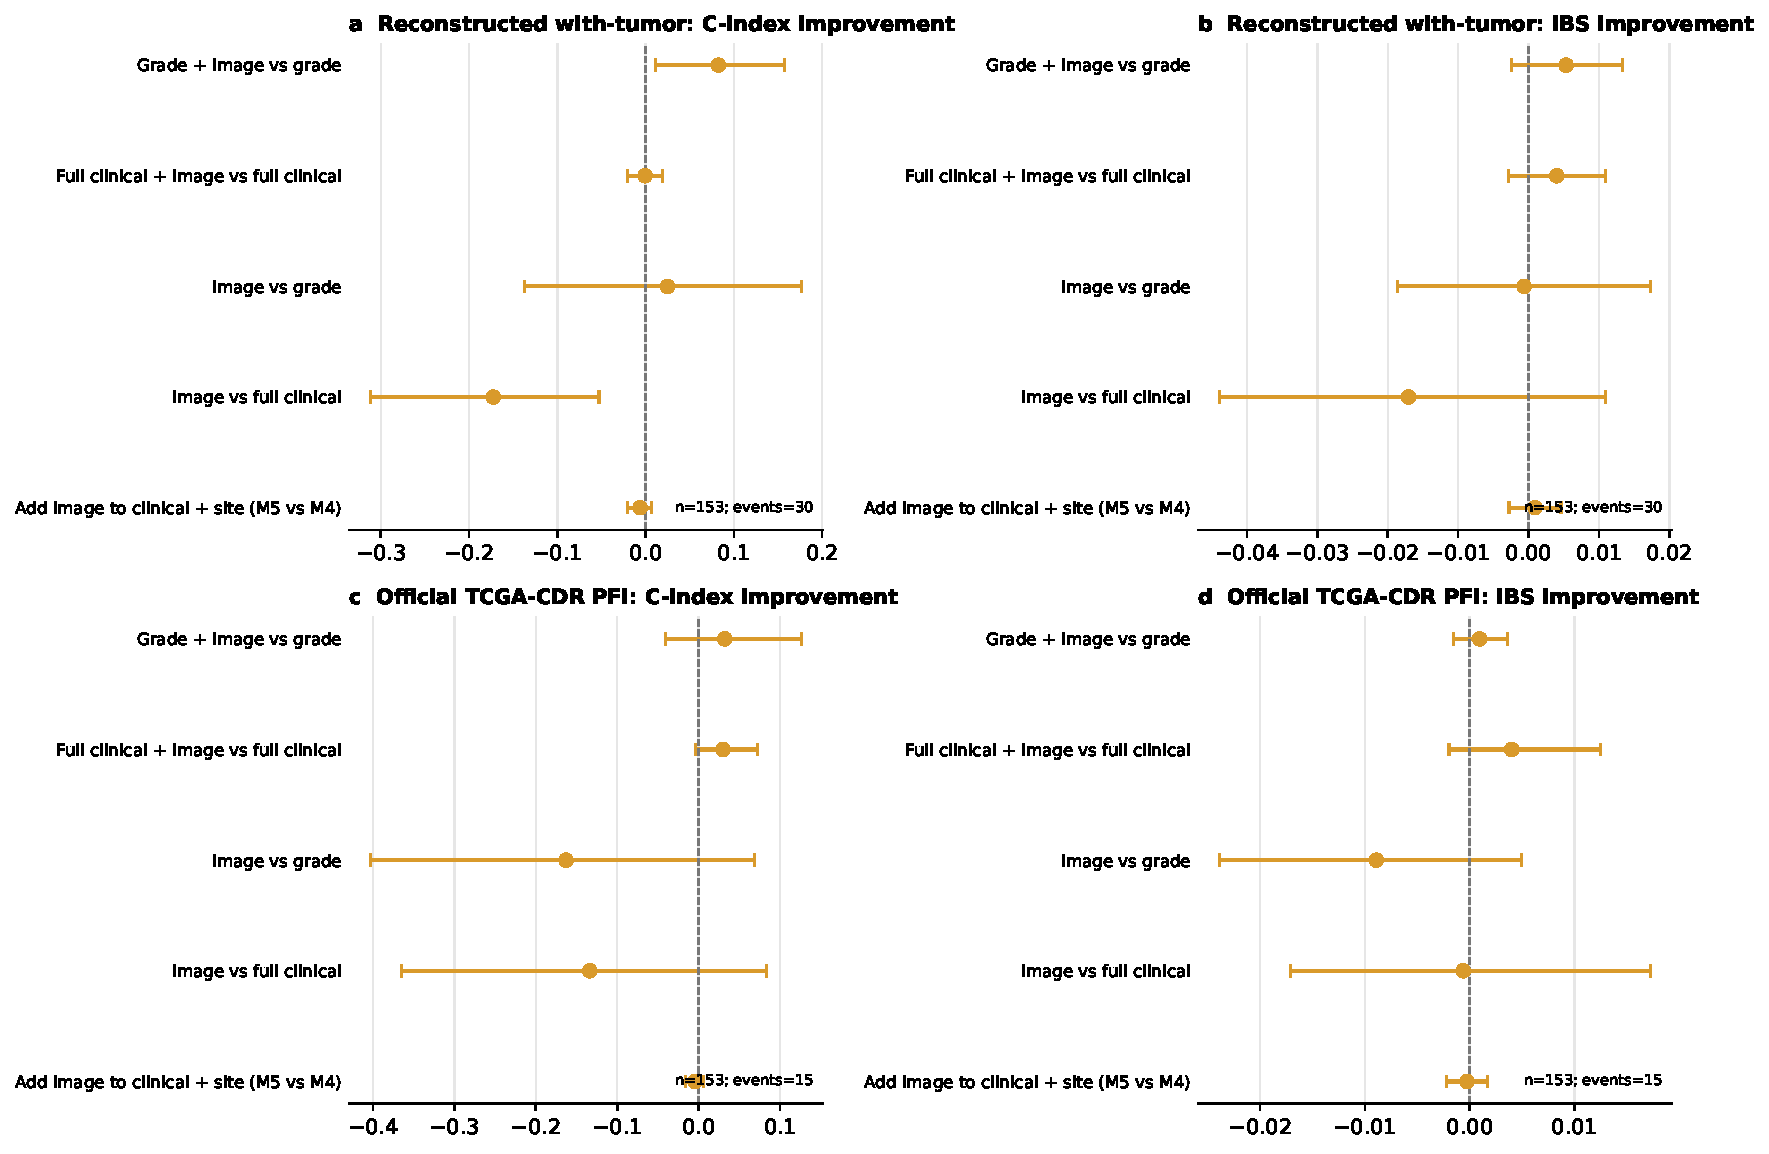
\includegraphics[width=\textwidth]{figures/fig6_outcome_contrasts.pdf}
\caption{\textbf{Complete paired outcome-comparison family across non-equivalent endpoints.}
Rows compare the image score with grade or fuller clinical references, or compare nested
clinical models, on the same patients and bootstrap draws. \textbf{a,b}, Reconstructed
with-tumor C-index and integrated-Brier-score (IBS) improvements. \textbf{c,d}, The same
comparisons for official TCGA-CDR PFI. Positive values favor the first, augmented, or more
complete model under the registered delta definition. These panels are comparator and
endpoint audits, not independent model validations; the difference between reconstructed
recurrence and official PFI is part of the result rather than a nuisance to be pooled.}
\label{fig:outcome-contrasts}
\end{figure}

\subsection{Representation audits bound sensitivity without selecting a universal model}
\label{sec:results-sensitivity}

\paragraph{Alignment question.}
Would the target-level interpretation change if the frozen encoder, physical image scale,
number of sampled tiles, or random tile sample changed?

\paragraph{Analysis frame.}
Six targets were evaluated across 12 encoder--scale--tile configurations and five sampling
seeds, yielding 360 correlated seed cells. The audit also contained 390 seed-matched scale,
encoder, and tile-budget contrasts.

\paragraph{Evidence test.}
For every target and configuration, the five seed-specific scores were compared with the
appropriate null---zero for Spearman correlation and 0.5 for AUROC or C-index. Paired
contrasts preserved the same seed when comparing encoder, scale, or tile budget. Grade,
phenotype, PTEN, and AR retained their direction across the observed configuration ranges.
SPOP ranges crossed the null in 8 of 12 configurations and recurrence in 1 of 12.

\paragraph{Interpretive boundary.}
These repeats reused cohorts, patients, folds, and representations. They reveal whether an
interpretation is dependent on analytic settings, but they are not independent replication
and do not support a universal CONCH-versus-Virchow ranking. Complete configuration ranges,
null crossings, and all 390 paired contrasts are reported in Supplementary Section S8;
Figures~\ref{fig:stability} and \ref{fig:setting-contrasts} expose their target-specific
ranges and contrast directions in the Main manuscript.

\paragraph{Qualification rule.}
Setting variation narrows a target's interpretation when its observed range crosses the
metric null or paired contrasts show material dependence. Stable direction across this grid
supports technical robustness within reused data only; external reproducibility still
requires a different cohort.

\begin{figure}[H]
\centering
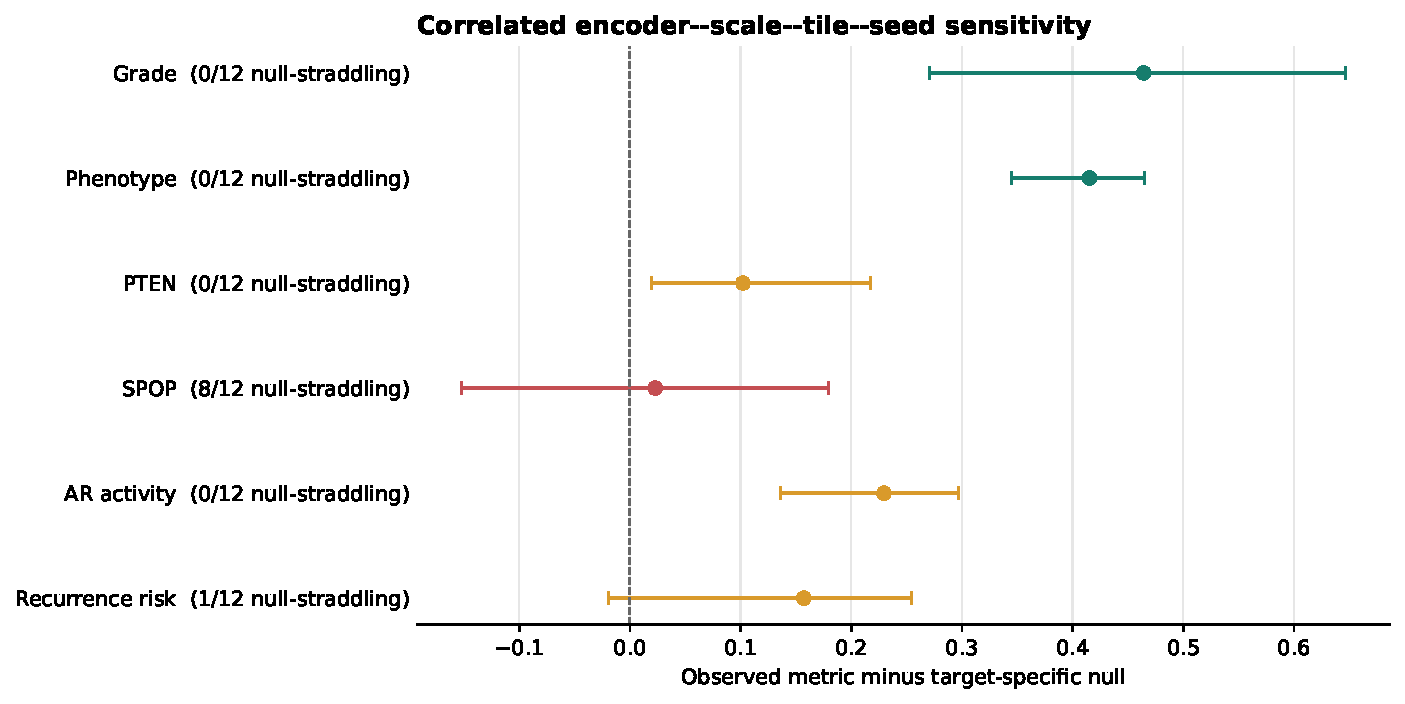
\includegraphics[width=\textwidth]{figures/fig4_representation_sensitivity.pdf}
\caption{\textbf{Target-specific representation and sampling sensitivity across all six axes.}
Observed five-seed ranges across 12 encoder--scale--tile configurations are shown relative
to each target's metric null. Counts record configurations whose observed seed range
straddled the null: 8 of 12 for SPOP and 1 of 12 for recurrence, versus retained direction
across the observed ranges for grade, phenotype, PTEN, and AR. All six axes are displayed on
their own metric scales; the 360 cells are correlated internal sensitivity settings rather
than independent validations or external transport tests.}
\label{fig:stability}
\end{figure}

\begin{figure}[H]
\centering
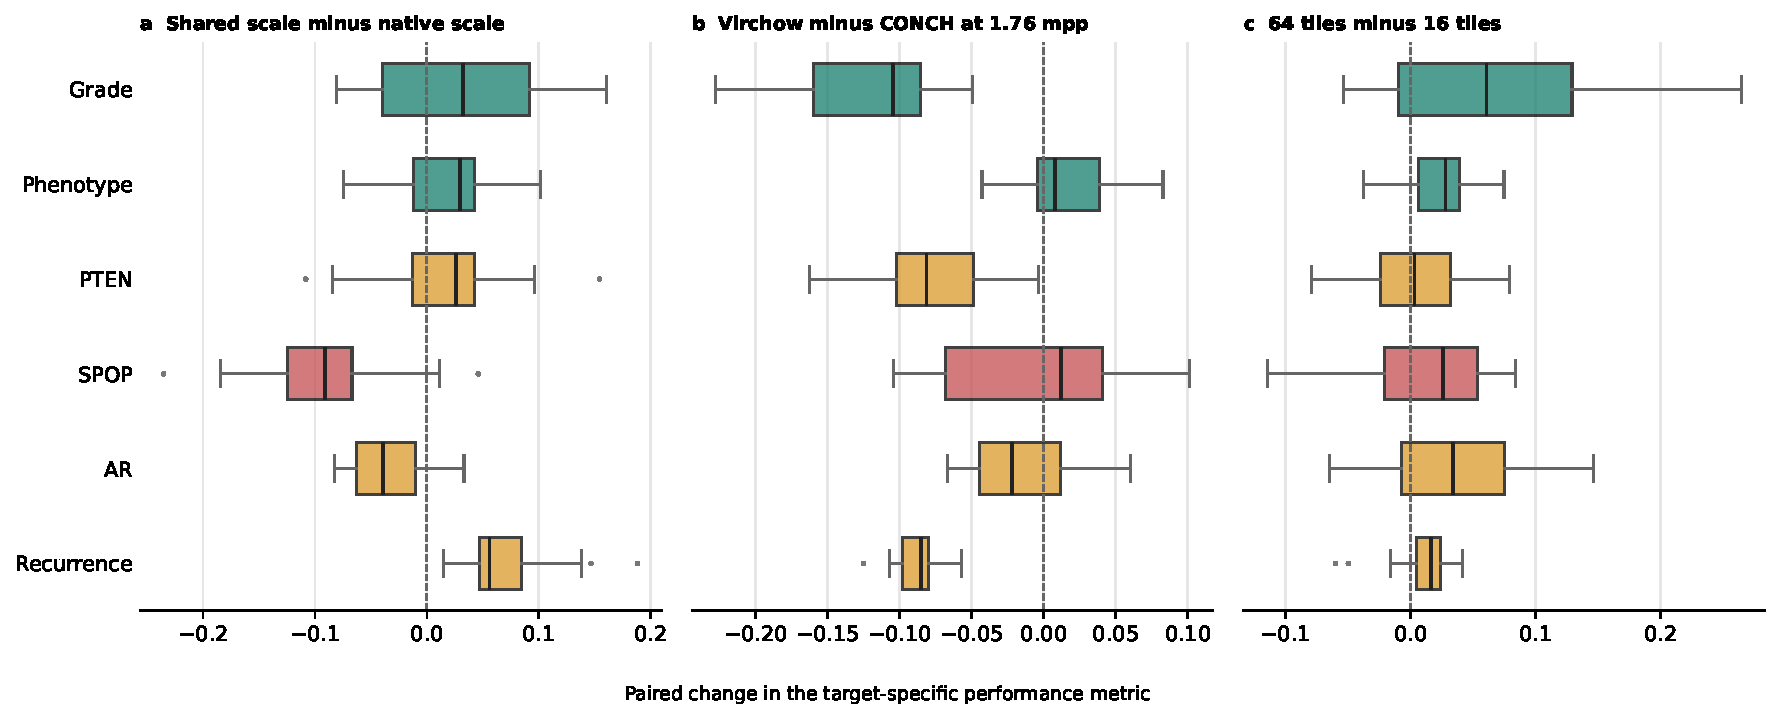
\includegraphics[width=\textwidth]{figures/fig5_setting_contrasts.pdf}
\caption{\textbf{Seed-matched encoder, physical-scale, and tile-budget contrasts.}
Each box summarizes paired performance changes for one target while preserving the same
sampling seed. \textbf{a}, Shared physical scale minus the encoder-native scale.
\textbf{b}, Virchow minus CONCH at the shared 1.76-micrometre-per-pixel scale.
\textbf{c}, 64 tiles minus 16 tiles per slide. The vertical null denotes no setting effect;
direction is specific to the named comparison and does not define a universally preferable
encoder or setting. All 390 comparisons reuse cohorts and folds.}
\label{fig:setting-contrasts}
\end{figure}

\subsection{ISUP provides the most developed extension from representation alignment to internal functional sensitivity}
\label{sec:results-functional-sensitivity}

The preceding analyses compared the representation-level evidence for all six axes. We next
asked how far one sufficiently recoverable axis could be advanced toward functional-use
testing. Grade/ISUP was the only target for which the current data and protocol supported
this extension; it was not treated as the sole or a priori organizing target of the study.

\paragraph{Alignment question.}
Does a locked AI risk head change when an ISUP-correlated direction is removed from its
input, and is that change larger than removing an equally large but randomly oriented part
of the representation?

\paragraph{Analysis frame.}
The exploratory FM6 frame comprised 392 TCGA-PRAD patients with 80 BCR events. CONCH and
Virchow remained frozen. For each encoder, a simple ridge probe learned an ISUP-correlated
direction, while a ridge-penalized Cox head learned BCR risk from the frozen representation.
``Locked head'' means that after this risk rule had been fitted, its coefficients were held
fixed while the ISUP-correlated direction was removed; the foundation model itself was not
retrained. The same patient-disjoint folds were used throughout.

\paragraph{Evidence test.}
ISUP was recoverable out of fold from both representations (Spearman $\rho=0.615$ for CONCH
and $0.658$ for Virchow). The full BCR heads had C-indices of 0.627 (0.553--0.694) and 0.632
(0.564--0.691), respectively. Removing the ISUP-correlated direction while keeping the head
fixed reduced concordance by 0.041 (0.011--0.073) for CONCH and 0.023 (0.007--0.040) for
Virchow. Both changes exceeded the respective variance-matched random-direction controls
($p=0.0099$ for each encoder). Thus the observation repeated across two distinct frozen
representations under the same internal analysis contract.

A protocol-locked clean rerun regenerated the FM6 analysis and figure outputs without
changing the cohort, embeddings, folds, seeds, endpoints, controls, thresholds, or
hyperparameters. All 20 protocol-defined nonvolatile output SHA-256 hashes matched the
pre-run baseline exactly, and the estimates, intervals, and gate decisions above were
unchanged. This establishes computational reproducibility of the internal experiment; it is
not an independent-cohort replication.

\paragraph{Interpretive boundary.}
The result supports sensitivity of these two internal heads to an ISUP-correlated subspace;
it does not prove that either head implements a human grading rule. When each head was
refitted after erasure, the full-minus-erased differences narrowed to 0.014
($-0.006$--0.035) for CONCH and 0.010 ($-0.003$--0.022) for Virchow, with intervals including
zero. This indicates that other embedding directions may compensate, so indispensable use
was not established. A limited comparison of ISUP plus the AI score against ISUP alone also
had intervals including zero (CONCH, $-0.000$, $-0.039$--0.039; Virchow, $-0.032$,
$-0.088$--0.025). That boundary check is insufficient to conclude that clinical increment
is absent; a dedicated, externally validated clinical-increment study was not performed.

The analysis used whole-tissue representations. A remediated tumor detector reached
specificity 0.810 on the already opened SICAP secondary test, which we accept as internal
technical evidence. However, sensitivity was only 0.562 and 0.679 on newly held-out PANDA
Karolinska and Radboud providers. Independent-domain sensitivity therefore remains
unresolved, and the present result is not described as tumor-specific or externally
transported functional use.

\paragraph{Qualification rule.}
Grade receives an \emph{internal exploratory functional-sensitivity} state because the
fixed-head effect was direction-specific, exceeded matched controls, and repeated across
CONCH and Virchow. It is the most developed example in the comparative map, but it is not
promoted to indispensable, external, mechanistic, or clinically incremental use. No residual
or unknown representation direction is evaluated as a new marker in this manuscript. In the
locked FM6 gate vocabulary, both encoders passed internal whole-tissue recoverability (R),
disease association (A), and exploratory functional sensitivity (U); external transport
(T) was not tested, and a strong H2 functional-use claim remained prohibited.

\subsection{The final alignment map distinguishes best-qualified, conditional, and unsuitable coordinates}

\paragraph{Alignment question.}
After combining all available axes, which targets are best-qualified candidates for shared
human--AI coordinates, and what evidence is still required?

\paragraph{Analysis frame and evidence test.}
We synthesized the registered primary, external, conditional, site, representation, and
endpoint rows without averaging unlike metrics or converting missing evidence into failure.

\paragraph{Interpretive boundary and qualification rule.}
The combined evidence supports a practical hierarchy. Grade and phenotype are the
best-qualified candidate shared coordinates because they were recoverable and directionally
transported. PTEN and AR can orient interpretation within the evaluated cohort, but their
independence and transport remain unresolved. SPOP is unsuitable under the frozen primary
design, and recurrence remains exploratory because its meaning changes with endpoint and
reference model. Grade alone also has internal exploratory functional-sensitivity evidence;
phenotype and the other targets do not. Table~\ref{tab:alignment-summary} summarizes these
decisions; expanded biological definitions are retained in Supplementary Section S1.

Figure~\ref{fig:human-ai-linkage} translates this hierarchy into a three-layer linkage map:
the clinically interpretable coordinate, the operational AI feature through which it was
tested, and the available evidence about downstream judgment. Here, an ``AI feature'' means
a probe-defined direction or score in the frozen embedding, not a localized gland, cell, or
latent unit with an independently established biological meaning. Grade/ISUP is the only
pathology coordinate that reaches the third layer through a locked-head intervention. The
other dashed links end at representation evidence, but for different reasons: phenotype is
currently blocked by the absence of same-cohort independent tumor-content truth; PTEN and AR
are feasible follow-up tests that were not run; SPOP lacks a qualified representation
feature; and recurrence is the prediction outcome rather than an input-feature erasure
target. This does not mean that only ISUP describes prostate cancer or that
all five remaining signals were equally visible. Phenotype had strong transported
representation evidence; PTEN and AR had conditional representation evidence; SPOP did not
yield a qualified representation feature; and recurrence produced an endpoint-sensitive
risk association. What is unique to ISUP is evidence that the tested BCR heads were
functionally sensitive to its correlated embedding direction.

\begin{figure}[H]
\centering
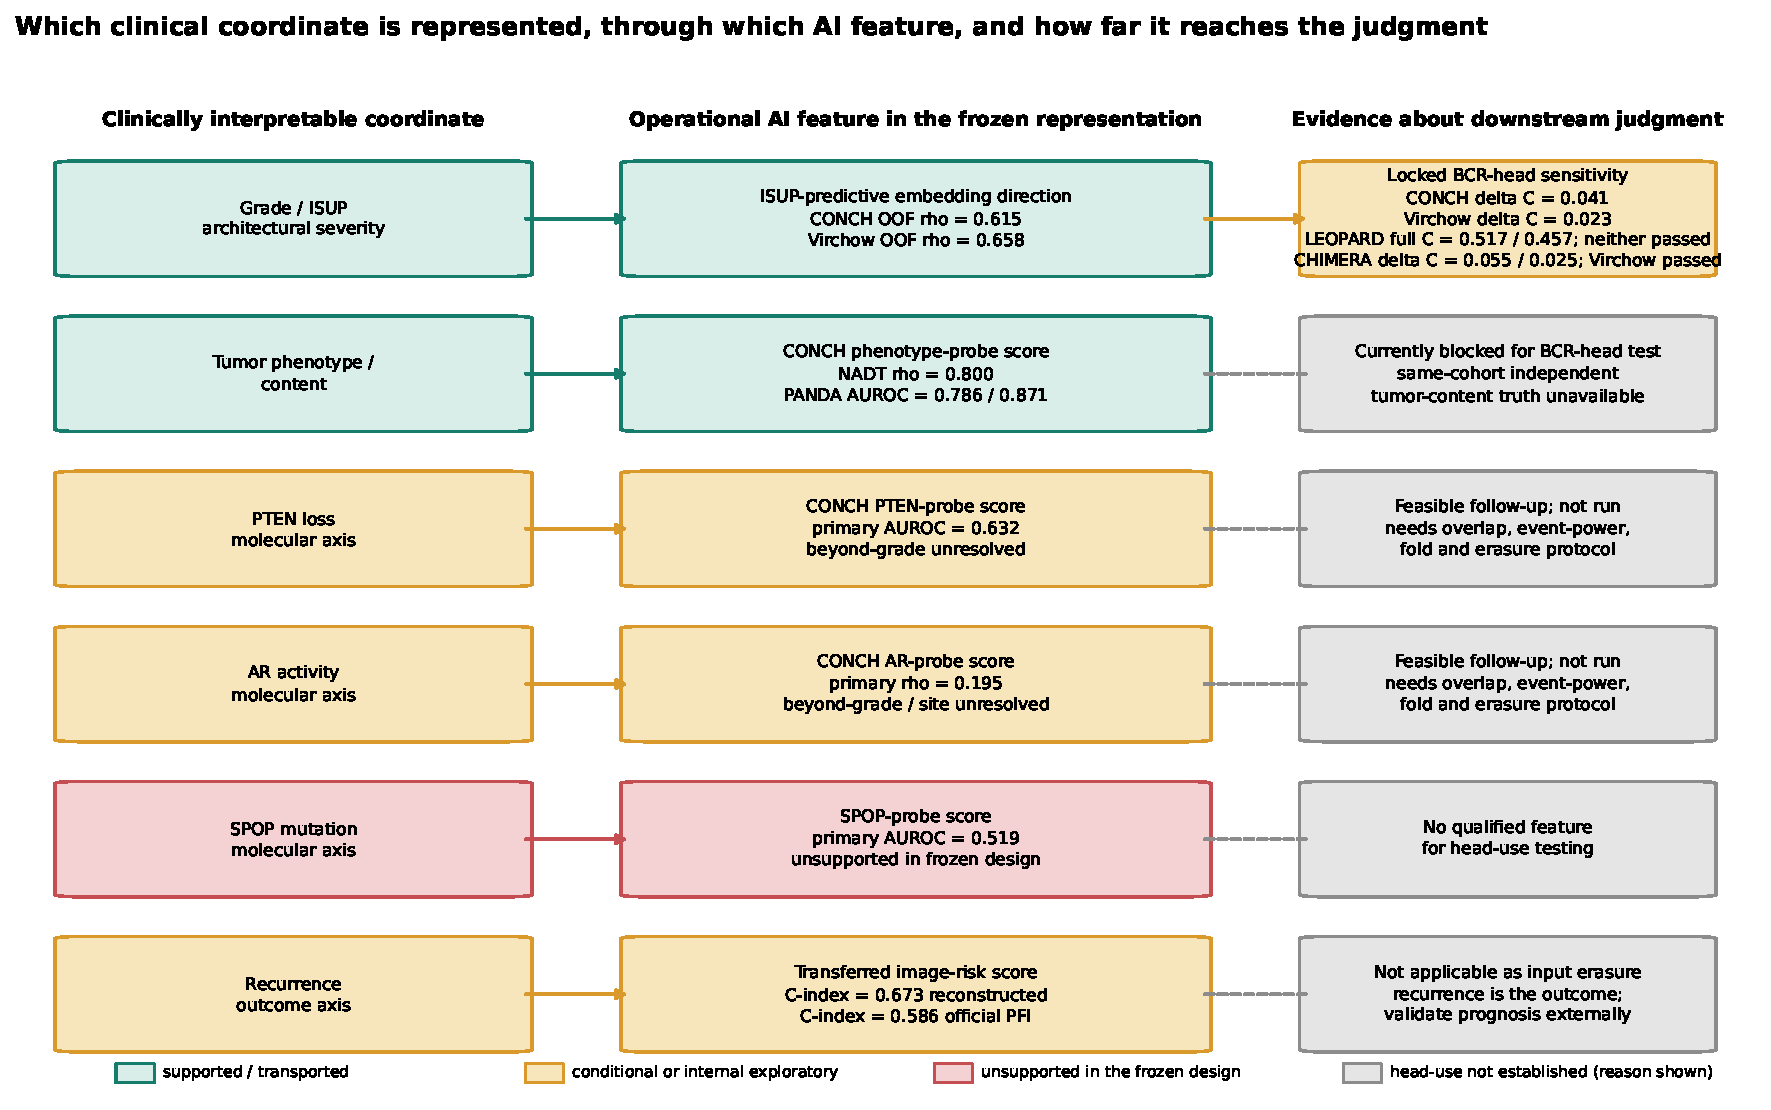
\includegraphics[width=\textwidth]{figures/fig7_human_ai_linkage_map.pdf}
\caption{\textbf{Human quantitative coordinate--AI feature--judgment linkage map.}
The left column names the clinically interpretable morphologic, molecular, or outcome axis.
The middle column identifies the operational representation feature used in this study: a
target-predictive probe direction or image-derived score. The right column shows whether
that feature was linked to a downstream judgment. Solid arrows denote an evaluated link;
dashed gray links denote that head use was not established, with the row-specific reason
written in the right-hand box. Only ISUP has internal locked-BCR-head erasure evidence,
repeated in CONCH and Virchow. This figure does not claim
that only ISUP characterizes cancer, that every other target is absent from the representation,
or that a probe direction is a localized histologic primitive. Phenotype is strongly
represented, PTEN and AR are conditionally represented, SPOP is unsupported, and recurrence
is an endpoint-sensitive outcome signal; these states must not be collapsed into one negative
category. The displayed coordinates do not completely explain an AI decision.}
\label{fig:human-ai-linkage}
\end{figure}
